\documentclass[fr]{../../../../../../eplexam}
\usepackage{../../../../../../eplcommon}
\usepackage{../../../../../../eplunits}

\newcommand{\degree}{^{\circ}}

\hypertitle[']{Automatique Linéaire}{6}{INMA}{1510}{2018}{Juin}{Majeure}
{Martin Braquet \and Margo Hauwaert}
{Denis Dochain}

\section{}

Soit le système ouvert en boucle ouverte suivant: 
\begin{equation*}
    \begin{cases} \dot{x}=Ax+Bu \\ y = Cx  \end{cases}
\end{equation*}

\begin{minipage}{0.4\textwidth}
$\begin{bmatrix}
-1&2&1\\
0&1&-1\\
-2&4&2\\
\end{bmatrix}=A$
\end{minipage}
\begin{minipage}{0.25\textwidth}
$\begin{bmatrix}
  0\\
  1\\
  0\\
\end{bmatrix} = B$
\end{minipage}
\begin{minipage}{0.3\textwidth}
$\begin{bmatrix}
  0 & 0 & 1\\
\end{bmatrix} = C$
\end{minipage}

Réécrivez la dynamique en séparant parties commandables et non commandables. 
Expliquez chaque étape de votre développement. 
Quelles conclusions tirez-vous? 
Justifiez votre réponse. 

\nosolution

\section{}

Soit un système dont la dynamique est décrite par le système suivant: 

\begin{equation*}
    G(s)=\frac{0.0054-0.015}{(s+0.325)(s^2-0.015s+0.0065)}
\end{equation*}

Soient les trois compensateurs suivants ($K_{p}, \tau_{i}, \tau_{d}$ sont positifs)
\begin{gather*}
\begin{aligned}
P &: C_{1}(s)=K_{p},  
  &
PI &: C_{2}(s)=K_{p}\frac{1+s\tau_{i}}{s\tau_{i}}, 
  &
PD &: C_{3}(s)=K_{p}(1+s\tau_{d}), 
\end{aligned}
\end{gather*}

Que pouvez-vous dire sur le système en boucle ouverte, en particulier en termes de pôles et zéros? Déterminez pour chaque compensateur si le système peut être stabilisé en boucle fermée par un retour unitaire de sortie. 

\nosolution

\section{}

Soit le système dynamique linéaire $\dot{x}=Ax+Bu$.

Sous conditions de stabilité de la paire $(A,B)$ et détectabilité de la partie $(Q,A)$ et avec connaissance de l'équation de Riccati algébrique:

\begin{equation*}
    A^TS+SA-SBR^{-1}B^TS+Q=0,
\end{equation*}
montrez que la commande 
\begin{equation*}
    u(t)=-R^{-1}B^TSx(t)
\end{equation*}
minimise la fonction quadratique 
\begin{equation*}
    \int_{0}^{\infty} (x^TQx+u^TRu)\:\mathrm{d} t.
\end{equation*}

\nosolution

\section{}

Soit un système en boucle fermée avec $$G(s)=\frac{1}{3}\frac{3-s}{s^3+2.5s^2+s}.$$ 

\begin{center}
 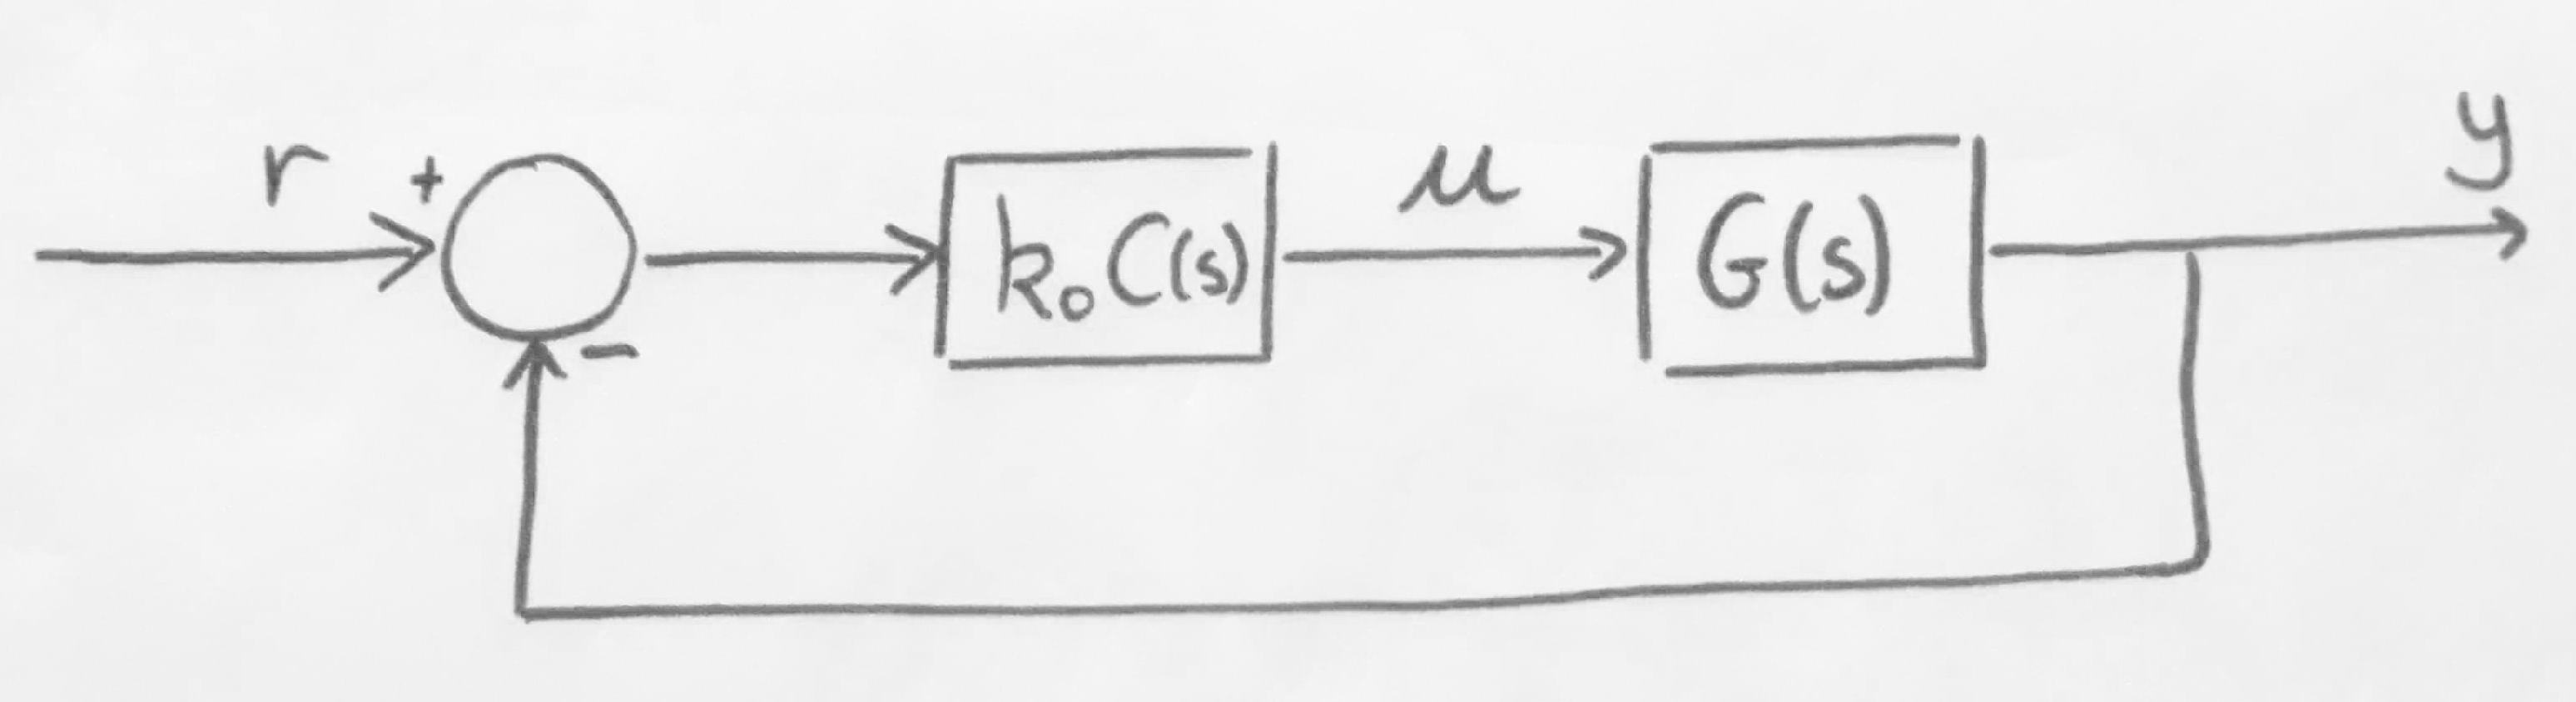
\includegraphics[scale=0.12]{q4.png}
\end{center}

Le diagramme de Bode a les caractéristiques suivantes\footnote{Un graphe du diagramme de Bode était disponible à l'examen.}:
\[
G_m=\SI{2.69}{dB} \mbox{ à } \SI{0.739}{rad/sec}
\]
\[
P_m=\SI{10.4}{deg} \mbox{ à } \SI{0.615}{ rad/sec}
\]
Déterminez un filtre à avance de phase $C(s)$ et la valeur du paramètre $k_0$ pour satisfaire aux spécifications suivantes: 
\[
    \phi_M = 45\degree \qquad\mathrm{pour}\qquad  \omega=\SI{0.5}{ rad/sec}
\]

\nosolution

\section{}

Soit un réacteur chimique continu avec 2 réactions isothermes en cascade 

\centerline{$A\rightarrow B$ et $B\rightarrow C$.} 
La dynamique du procédé peut être caractérisée par les équations de bilan de masse suivantes: 

\[
\fdif{C_A}{t} = \frac{q}{V}C_{A,in}-\frac{q}{V}C_{A}-k_{01}C_A
\]
\[
\fdif{C_B}{t} = \frac{-q}{V}C_{B}+b\,k_{01}C_A-k_{02}C_B
\]
où $q, C_A, C_{A,in}, C_B, V, k_{01}, k_{02}$ et $b$ sont respectivement 
\begin{itemize}
  \item le débit volumique d'entrée $(m^3/h)$,
  \item la concentration du réactif A dans le réacteur et sans l'alimentation $(g/L)$,
  \item la concentration de B dans le réacteur $(g/L)$,
  \item le volume du réacteur $(m^3)$,
  \item les constantes cinétiques de la première et de la deuxième réaction $(h^{-1})$,
  \item le coefficient stoechiométrique associé à la première réaction
\end{itemize}  
L'entrée de commende est $C_{A,in}$.

\begin{enumerate}
  \item Vous avez accès à la mesure $C_B$ mais pas à celle de $C_A$, que vous souhaitez déterminer en temps réel en utilisant un observateur de Luenberger, dont vous souhaitez fixer les pôles. Donnez les équations de l'observateur dans ce cas. 
  \item Vous êtes dans la situation inverse où vous mesurez $C_A$ mais pas $C_B$ et vous utilisez la même approche qu'au point 1 pour synthétiser un observateur de Luenberger. Donnez les équations de l'observateur dans ce cas. 
  \item Comparez les 2 observatuers en termes de performances dynamiques. Justifiez votre réponse. 
  \item Donnez les valeurs des gains de l'observateur $K$ de Kaman dans le premier cas, sachant que l'équation de Ricatti et le gain $K$ s'écrivent ainsi:
    \[
    0=-RC^TCR+RA^T+AR
    \]
    \[
    K=RC^T
    \]
    où $R=R^T$ et $A$ et $C$ sont des matrices d'état et de sortie du système dynamique linéaire. 
\end{enumerate}


\nosolution

\section{}

Soit le système en boucle fermée suivant: 

\begin{center}
 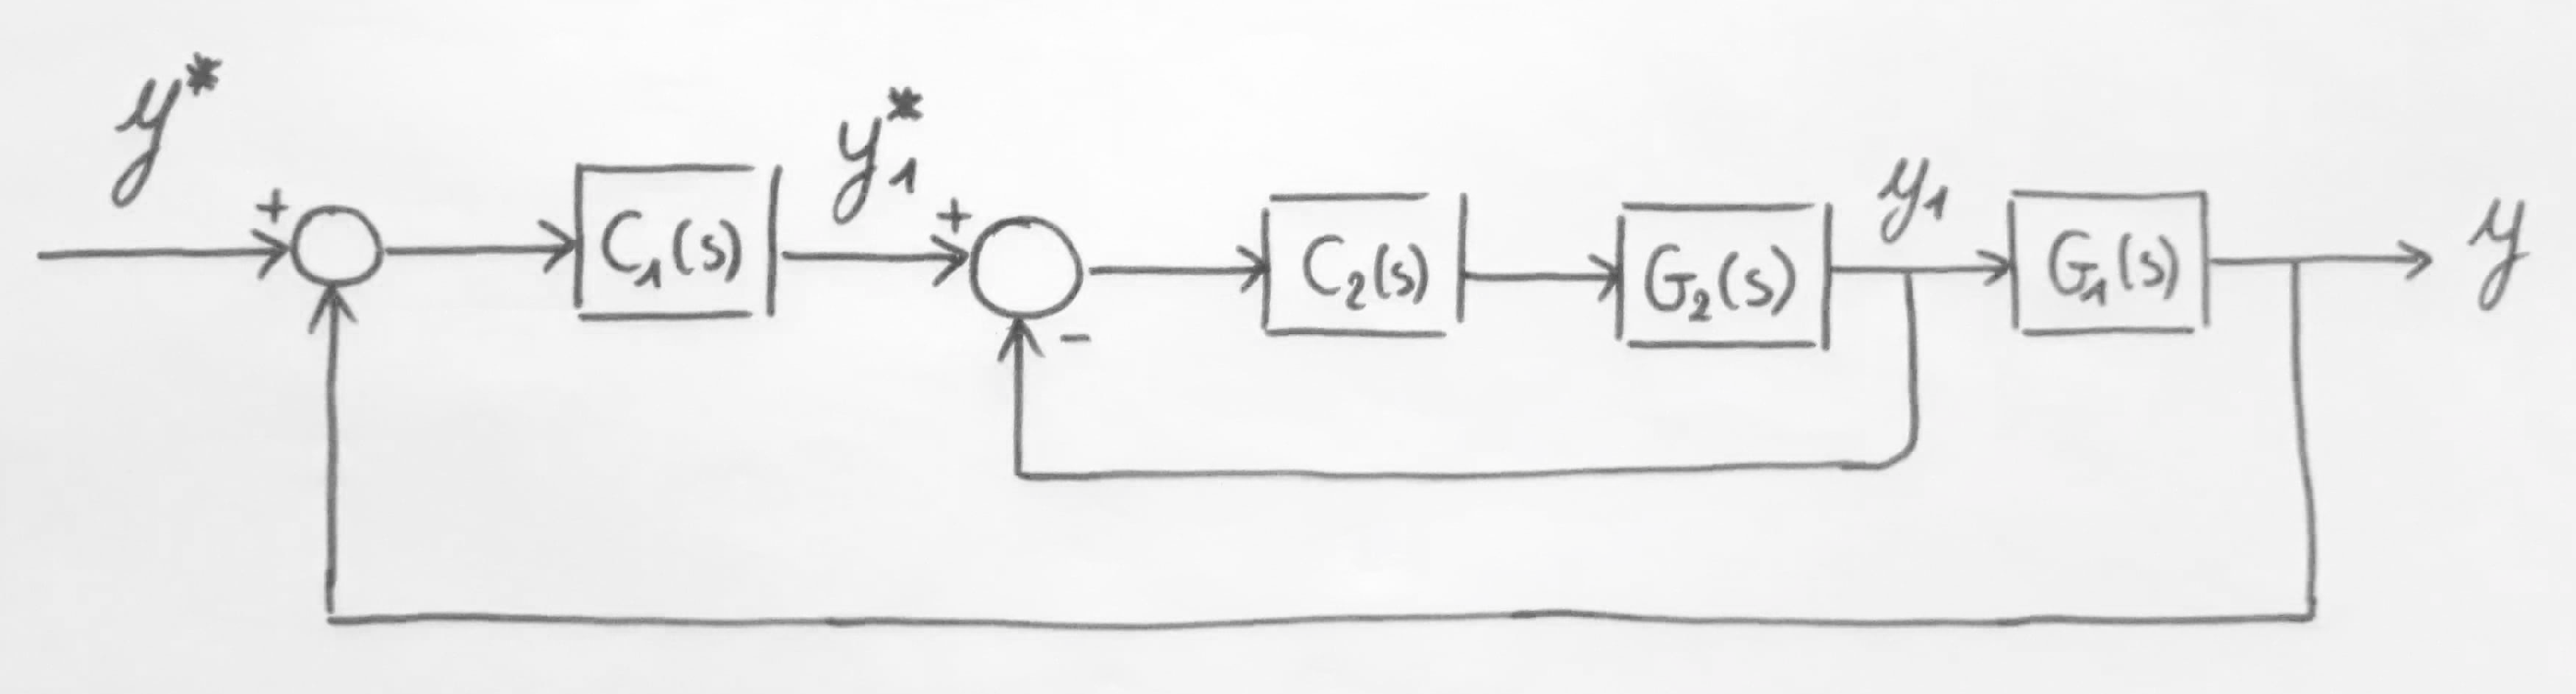
\includegraphics[scale=0.10]{q6.png}
\end{center}

avec 
\begin{equation*}
     C_1(s)=K_{p1}\frac{1+s\tau_{i1}}{s\tau_{i1}} \qquad C_2(s)=K_{p2} \qquad G_1(s)=\frac{4}{4S+1} \qquad G_2(s)=\frac{5}{s+1}
\end{equation*}

\begin{enumerate}
    \item Comment s'appelle cette structure? Quel est son intérêt? Quels sont ses avantages et inconvénients? 
    \item Déterminez les valeurs de $K_{p1}, K_{p2}, \tau_{i1}$ de manière à avoir une dynamique en boucle fermé avec seulement deux pôles en -4 et -5.
    \item Cette structure de commande permet-elle d'annuler l'erreur statique? Justifiez vos réponses. 
\end{enumerate}

\nosolution

\end{document}
